\documentclass[12pt,a4paper,fleqn]{article}
\title{Progress Report}
\author{Syed Ahmad Raza}
\date{2017.12.06}
\usepackage{mathtools}
\usepackage{graphicx}
\usepackage{color}          % for color eps output
% \usepackage{afterpage}
\usepackage{float}          % to force a figure placement with [H] command
\usepackage{enumitem}
\usepackage{newtxtext}
\usepackage{newtxmath}
%\usepackage{layouts}       % for: \printinunitsof{in}\prntlen{\textwidth}

\begin{document}
\maketitle
%\tableofcontents
%\pagebreak

\section{Finite Volume Method for 2D flows}

\subsection{Troubleshooting to reduce error of numerical solution}
The code was modified to use maximum value of pressure and velocity when testing convergence of the solution.

Velocity profiles are presented here at a fixed set conditions for the three different velocity schemes. The analysis was repeated with an increasing number of grids and at different Reynolds numbers.

\subsection{Vertical grid points, \(ny=10\)\\
    Reynolds number, \(Re=10\)}

\begin{figure}[H]
    \centering
    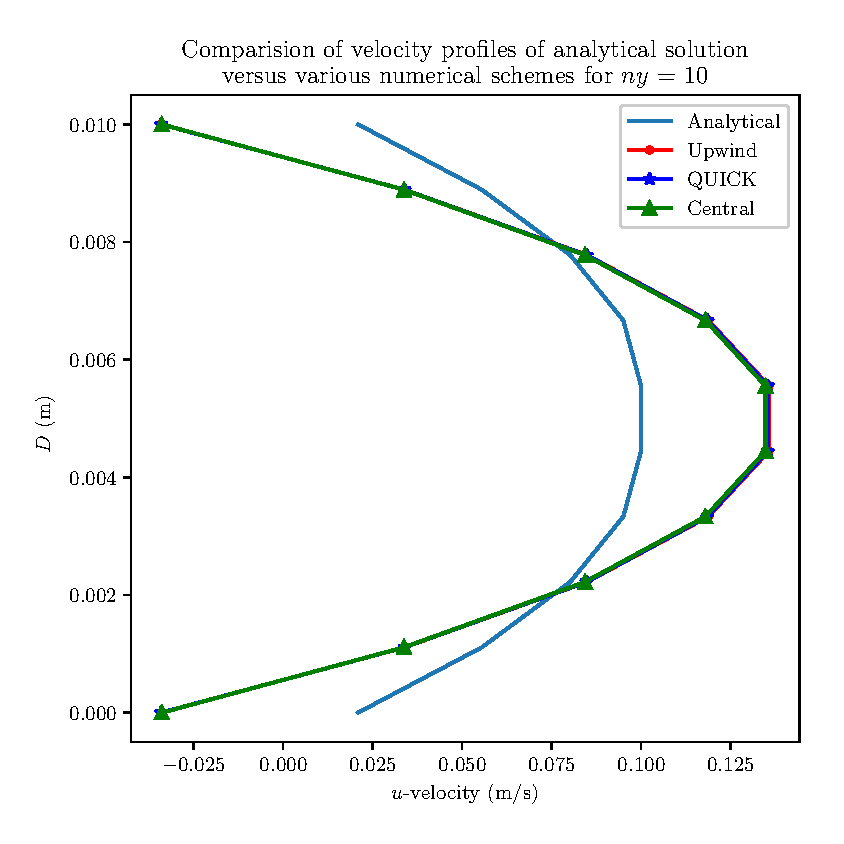
\includegraphics[width=\textwidth]{ny-10_profilesComparison.eps}
    \caption{Velocity profiles of numerical solutions using different velocity schemes is compared with that of analytical solution, for 10 vertical grid points at \(Re = 10\).}
    \label{fig:ny-10_profilesComparison}
\end{figure}

\subsection{Vertical grid points, \(ny=30\)\\
    Reynolds number, \(Re=10\)}

\begin{figure}[H]
    \centering
%    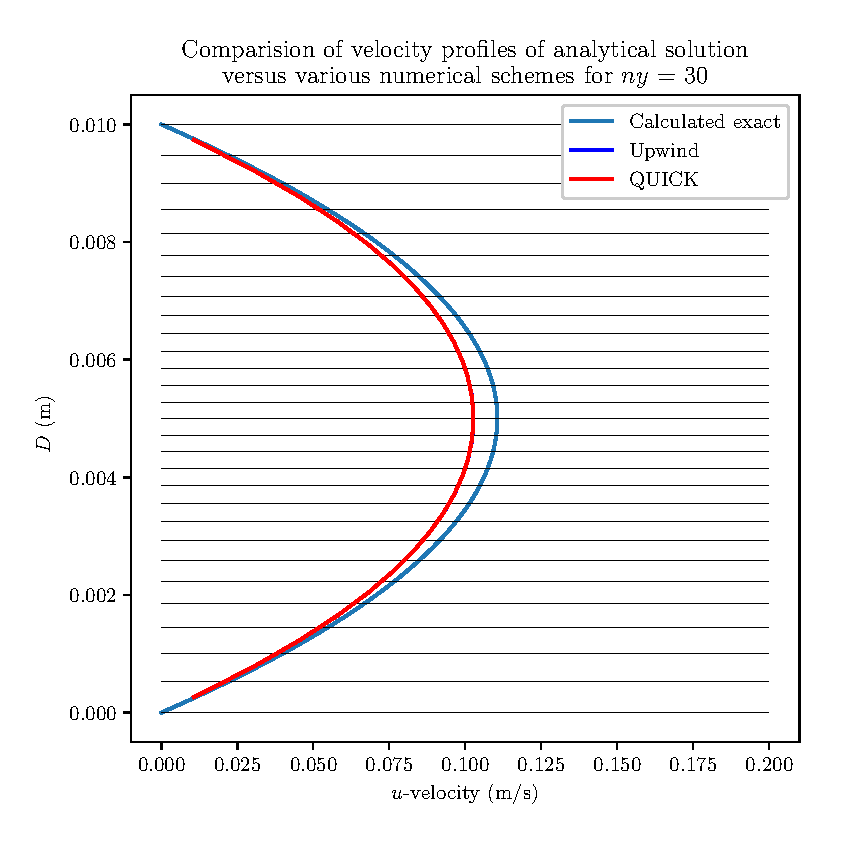
\includegraphics[width=\textwidth]{ny-30_profilesComparison.eps}
    \caption{Velocity profiles of numerical solutions using different velocity schemes is compared with that of analytical solution, for 30 vertical grid points at \(Re = 10\).}
    \label{fig:ny-30_profilesComparison}
\end{figure}

\subsection{Vertical grid points, \(ny=10\)\\
    Reynolds number, \(Re=100\)}

\begin{figure}[H]
    \centering
%    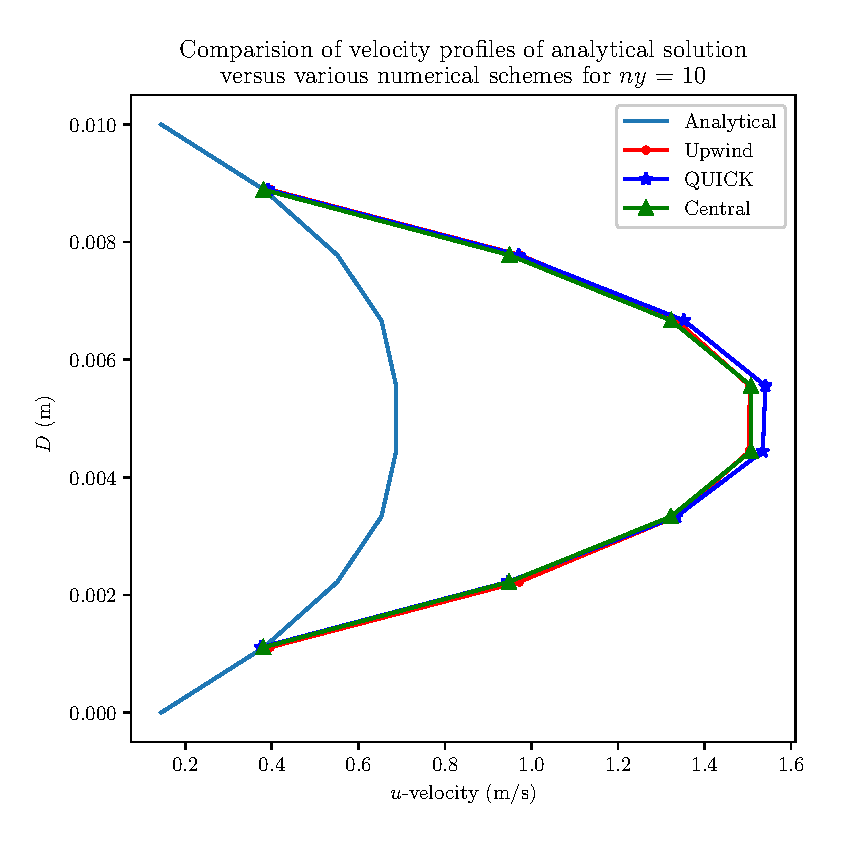
\includegraphics[width=\textwidth]{Re-100_ny-10_profilesComparison.eps}
    \caption{Velocity profiles of numerical solutions using different velocity schemes is compared with that of analytical solution, for 10 vertical grid points at \(Re = 100\).}
    \label{fig:Re-100_ny-10_profilesComparison}
\end{figure}

\subsection{Substitutions for velocities in the convective terms}
A simple mean is used for the velocities $u_n, u_s, v_e$ and $v_w$,
\begin{equation*}
\begin{aligned}
u_n &= u_{i,j} + \frac{u_{i,j+1} - u_{i,j}}{(y_{j+2}-y_j)/2}\\
u_s &= u_{i,j} - \frac{u_{i,j} - u_{i,j-1}}{(y_{j+1}-y_{j-1})/2}
\end{aligned}
\qquad\qquad
\begin{aligned}
v_e &= v_{i,j} + \frac{v_{i+1,j} - v_{i,j}}{(x_{i+2}-x_i)/2}\\
v_w &= v_{i,j} - \frac{v_{i,j} - v_{i-1,j}}{(x_{i+1}-x_{i-1})/2}
\end{aligned}
\end{equation*}

For rest of the velocities in the convective terms, namely $u_e, u_w, v_n$ and $v_s$, the following three schemes were used:
\begin{enumerate}
\setlength\itemsep{0em}
\item Upwind scheme
\item Central difference scheme
\item Quadratic Upwind Interpolation for Convective Kinematics (QUICK)
\end{enumerate}

\paragraph{Upwind scheme}\mbox{}\\
For positive velocities,
\begin{equation*}
\begin{aligned}
u_e = u_{i,j}\\
u_w = u_{i-1,j}
\end{aligned}
\qquad\qquad
\begin{aligned}
v_n = v_{i,j}\\
v_s = v_{i,j-1}
\end{aligned}
\end{equation*}
For negative velocities,
\begin{equation*}
\begin{aligned}
u_e = u_{i+1,j}\\
u_w = u_{i,j}
\end{aligned}
\qquad\qquad
\begin{aligned}
v_n = v_{i,j+1}\\
v_s = v_{i,j}
\end{aligned}
\end{equation*}

\paragraph{Central scheme}
\begin{equation*}
\begin{aligned}
u_e = \frac{u_{i,j} + u_{i+1,j}}{2}\\
u_w = \frac{u_{i-1,j} + u_{i+1,j}}{2}
\end{aligned}
\qquad\qquad
\begin{aligned}
v_n = \frac{v_{i,j} + v_{i,j+1}}{2}\\
v_s = \frac{v_{i,j-1} + v_{i,j}}{2}
\end{aligned}
\end{equation*}

\paragraph{QUICK scheme}\mbox{}\\
For positive velocities,
\begin{equation*}
\begin{aligned}
u_e = \tfrac{6}{8}u_{i,j} + \tfrac{3}{8}u_{i+1,j} - \tfrac{1}{8}u_{i-1,j}\\
u_w = \tfrac{6}{8}u_{i-1,j} + \tfrac{3}{8}u_{i,j} - \tfrac{1}{8}u_{i-2,j}
\end{aligned}
\qquad\qquad
\begin{aligned}
v_n = \tfrac{6}{8}v_{i,j} + \tfrac{3}{8}v_{i,j+1} - \tfrac{1}{8}v_{i,j-1}\\
v_s = \tfrac{6}{8}v_{i,j-1} + \tfrac{3}{8}v_{i,j} - \tfrac{1}{8}v_{i,j-2}
\end{aligned}
\end{equation*}
For negative velocities,
\begin{equation*}
\begin{aligned}
u_e = \tfrac{6}{8}u_{i+1,j} + \tfrac{3}{8}u_{i,j} - \tfrac{1}{8}u_{i+2,j}\\
u_w = \tfrac{6}{8}u_{i,j} + \tfrac{3}{8}u_{i-1,j} - \tfrac{1}{8}u_{i+1,j}
\end{aligned}
\qquad\qquad
\begin{aligned}
v_n = \tfrac{6}{8}v_{i,j+1} + \tfrac{3}{8}v_{i,j} - \tfrac{1}{8}v_{i,j+2}\\
v_s = \tfrac{6}{8}v_{i,j} + \tfrac{3}{8}v_{i,j-1} - \tfrac{1}{8}v_{i,j+1}
\end{aligned}
\end{equation*}

\end{document}
